\chapter{Introducción}
\graphicspath{{./figs/01_intro/}}
\chapterquote{La destrucción es obra de una tarde. La creación es obra de una vida.}{Kamahl, acólito druida}
\section{Motivación}\label{S:motivacion}
Dentro de la multitud de materiales existentes, los sólidos cristalinos son aquellos que tienen más impacto en el desarrollo de nuestra vida cotidiana. 
Los sólidos cristalinos son materiales que están constituidos por cristales, que son arreglos periódicos de átomos. 
Dado que en el transcurso de este trabajo sólo se hablará de sólidos cristalinos, cuando se hable de sólido, material o muestra, siempre se sobreentenderá que se está hablando de un sólido cristalino. 
La unidad básica de un cristal es la denominada celda unidad, que se repite en las tres dimensiones del espacio, dándole al cristal una simetría de traslación. 
Según el principio de Neumann[ref], las propiedades básicas de un sólido cristalino están determinadas en primer lugar por la de la celda unidad, y serán en general anisotrópicas, es decir dependerán de la orientación de dicha celda respecto a un cierto sistema de referencia.
En un dado sólido, puede ocurrir que todos sus cristales tienen la misma orientación, en cuyo caso se dice que ese material es un mono-cristal. Si por el contrario, el sólido está constituido por cristales orientados en cualquier dirección, y todas las orientaciones se encuentran igualmente representadas, se dice entonces que el material es un poli-cristal. 
En el caso más general se tendrá una situación intermedia entre un mono-cristal y un poli-cristal, es decir, los cristales tendrán una o más orientaciones preferenciales y habrá una cierta distribución en dichas orientaciones, lo que constituirá la textura de dicho material. La textura de un material es el segundo factor que condicionará la anisotropía de las propiedades macroscópicas de un sólido cristalino.

Dar algunos ejemplos de relaciones entre textura y propiedades mecanicas.

En este trabajo se estudia la anisotropía de distintas aleaciones metálicas, buscando relaciones entre las deformaciones mecánicas sufridas por las muestras, su textura y los defectos acumulados por las mismas.

\cite{Mainprice2011}
\section{Difracción de Rayos X}\label{S:DRX}
Los rayos X son una herramienta de vital importancia para el estudio de los materiales cristalinos. 
En la difracción de Rayos X (DRX), un haz monocromático de de rayos X de longitud de onda $\lambda$ incide sobre una dada muestra (Fig. \ref{fig:Bragg}). 
Si el cristal es infinito y está libre de cualquier tipo de distorsiones, para una dada familia de planos ${hkl}$, habrá interferencia constructiva para los haces salientes que cumplan con la condición de Bragg[ref]:
\begin{equation}
  2 \ d_{hkl} \ \sin(\theta_{B}) \ = \ n \ \lambda
  \label{eq:Bragg}
\end{equation}
\noindent
siendo $d_{hkl}$ la distancia interplanar de la familia de planos $\{hkl\}$, 2$\theta_{B}$ el ángulo formado entre el haz incidente y el haz reflejado y $n$ el número de orden de difracción. 

Hay que pensar en el planteo mas riguroso, usando los vectores K, porque lo voy a necesitar para explicar williamson hall

\nomenclature{$\lambda$}{Longitud de onda}
\nomenclature{$d_{hkl}$}{Distancia interplanar para la familia de planos $hkl$}
\nomenclature{$\theta_B$}{Ángulo de Bragg}
\nomenclature{XRD}{Difracción de Rayos X}
\begin{figure}[htb!]
  \centering
  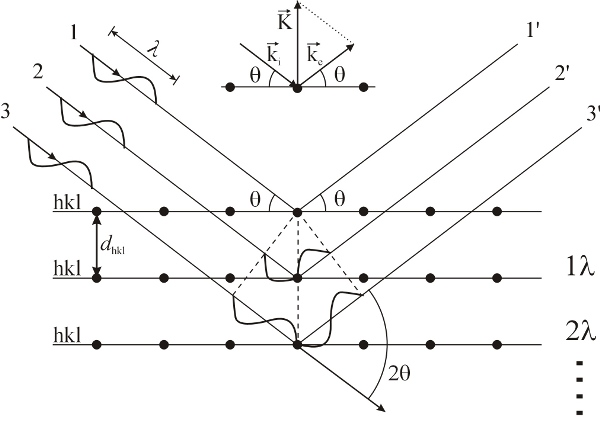
\includegraphics[width=\imsize]{BraggLaw}
  \caption{Ley de Bragg}
  \label{fig:Bragg}
\end{figure}

Una consecuencia de la ley expresada en la Ec. \ref{eq:Bragg} es que para un cierto haz incidente habrá reflexiones cuyas distribución de intensidades serán funciones deltas de Dirac[ref], con intensidad infinita para el ángulo $\theta_{B}$ e intensidad nula para los ángulos $\theta$ que no cumplan con la condición de Bragg. Como resultado, los "picos" de difracción tendrán un ancho nulo. 
Si, como ocurre en la práctica, el número de planos que contribuyen a la reflexión es finito, la distribución angular de intensidades tendrán un ancho y altura finitos, y lo mismo ocurrirá si la red de átomos tiene distorsiones, es decir, si los átomos no se encuentran en un arreglo perfectamente periódico. 
En un experimento de DRX real aparecerán además otras contribuciones que ensancharán los picos de difracción. 
Por ejemplo, el haz incidente no será puntual ni estará constituido por haces completamente paralelos, sino que tendrá un tamaño finito y estará comprendido entre haces que tendrán cierta divergencia angular.
Además, el haz no será completamente monocromático, sino que estará integrado por rayos X con longitudes de onda en un intervalo $(\lambda \ \pm \ \Delta \lambda)$. 
Todos estos factores contribuirán a que haya haces difractados en las vecindades de $\theta_{B}$, aumentando el ancho de los picos de difracción. Una parte importante de esta tesis se tratará de obtener información acerca de la microestructura de los materiales a partir del ensanchamiento de los picos de difracción, por lo que la correcta clasificación y cuantificación de los efectos instrumentales será motivo de discusión permanente en los capítulos siguientes.

\subsection{Estudios de ancho de pico}\label{SS:DRX-LPA}
Si no se tienen en cuenta los diferentes efectos instrumentales se puede afirmar que, a partir del estudio del ensanchamiento y la forma de los perfiles de intensidad de los picos de medidos en un experimento de DRX, es posible obtener información acerca de la cantidad y tipo de defectos presentes en un material, así como información microestructural como el tamaño promedio de los dominios coherentes de difracción (cristalitas).
Al conjunto de técnicas y métodos del campo de la cristalografía que utilizados para obtener este tipo de información se los conoce como Estudios de Ancho de Pico, o LPA, por sus siglas en inglés (Line Profile Analysis).
Aunque el término LPA fue acuñado muchos años después, la técnica, aunque rudimentaria, es tan antigua como los primeros experimentos de DRX, y fue implementada independientemente por Hull en Estados Unidos y Debye y Scherrer en Alemania. Mientras investigaba el tamaño de partículas de oro y plata en sistemas coloidales, Scherrer incluyó la ecuación que luego llevaría su nombre[ref]:

\begin{equation}
  H \ = \ 2 \sqrt{\frac{\ln(2)}{\pi}} \ \frac{\lambda}{L \ \cos(\theta_B)}
  \label{eq:Scherrer}
\end{equation}
\noindent
Donde $H$ denota el ancho del pico a la mitad de su intensidad máxima (también abreviado FWHM), $L$ es la longitud característica de la cristalita y el factor numérico se usa para convertir $H$ al ancho integral del pico, suponiendo que el mismo tiene forma de gaussiana. 
Los trabajos que siguieron se dedicaron a mejorar las estimaciones de tamaño y forma de las cristalitas. 
En el año 1938 [ref] Jones señaló que el perfil de intensidades medido en un experimento de DRX, $I_{exp}$, es la convolución del perfil $I_{muestra}$ que se obtendría de la muestra y el debido a todos los efectos instrumentales, $I_{inst}$, es decir:
\begin{equation}
  I_{exp} \ = \ I_{muestra} \ \otimes \ I_{inst}
  \label{eq:conv}
\end{equation}
\noindent
De esta manera, Jones logró remover las contribuciones de las líneas $K\alpha_2$ de la radiación del cobre en las mediciones de tamaño de cristalita. 
En el año 1949 Hall[ref] usó la formulación de Stokes y Wilson [ref] para proponer un método para separar las contribuciones de los efectos de tamaño de cristalita y de deformación de la red cristalina, basándose en el hecho de que cada contribución tiene una variación característica con el orden de difracción ${hkl}$.
Al graficar el ancho integral de cada pico de difracción en función de $K$, los puntos se acomodan en una recta cuya pendiente está relacionada con el nivel de deformación de la red, y cuya ordenada al origen es el recíproco del tamaño de cristalita promedio ($D$):
\begin{equation}
  \beta \ \cos\left(\frac{\theta}{\lambda}\right) \ = \frac{1}{D} \ + \ \left(\frac{\epsilon}{2}\right) \ K
  \label{eq:WHPlot}
\end{equation}
\noindent
siendo $\epsilon$ una cantidad que es proporcional a la distorsión de la red cristalina y $\beta$ es el ancho integral de cada reflexión. La primera versión del método de Williamson-Hall, que es como se llamó a la aplicación de la Ec. \ref{eq:WHPlot}, se basa en la suposición de que los picos de difracción tienen un perfil lorentziano. Si los perfiles tienen un carácter gaussiano, muchos pasos en la deducción son iguales, pero el resultado final es lo que se denomina la forma cuadrática de la ecuación de Williamson-Hall[ref]:
\begin{equation}
  (\beta \ \cos\left(\frac{\theta}{\lambda}\right))^2 \ = (\frac{1}{D})^2 \ + \ (\left(\frac{\epsilon}{2}\right) \ K)^2  (chequear con el paper Ungar)
  \label{eq:WHPlot2}
\end{equation}
\noindent
En el año 1949, Warren y Averbach [ref] también utilizaron la formulación de Stokes y Wilson para derivar otro método para separar las contribuciones de distorsión y tamaño al ensanchamiento de los picos de rayos X. 
El método de Warren-Averbach se basa en el hecho de que la transformada de Fourier de la convolución de dos funciones es simplemente el producto de las transformadas de Fourier de dichas funciones[ref].
Por lo tanto, como el perfil de intensidades $I_{muestra}$ es la convolución del perfil obtenido por las contribuciones de tamaño $I_{T}$ y distorsión $I_{D}$, los coeficientes de Fourier del perfil de línea de la muestra $A_n$ son el producto de los coeficientes de tamaño $A_n^T$ y distorsión $A_n^D$:
\begin{equation}
  A_n \ = \ A_n^T \ A_n^D
  \label{eq:FCoeff}
\end{equation}
\noindent
En este caso, si se supone que las cristalitas son de forma esférica y que su distribución de tamaño de de tipo lognormal[ref] y se supone un perfil de deformación de tipo gaussiano, se puede llegar a la ecuación que se emplea cuando se aplica el método de Warren-Averbach[chequear]:
\begin{equation}
  \ln(A_n(l)) \ = \ \ln(A_n^T) \ - \ 2 \pi^2 n^2 l^2 \ <e^2>
  \label{eq:WAPlot}
\end{equation}
\noindent
En la Ec. \ref{eq:WAPlot}, $l$ es el orden de una dada reflexión, $<e^2>$ es la deformación media de la red cristalina y el resto de los símbolos son acordes a las definiciones anteriores.


\nomenclature{$H$ o $FWHM$}{Ancho de pico a media altura. También abreviado como FWHM por sus siglas en inglés (Full Witdth at Half Maximum).}
\nomenclature{$L$}{Longitud característica de la cristalita.}
\nomenclature{$<e^2>$}{Deformación cuadrática media de la red cristalina}
\nomenclature{$l$}{Orden de reflexión}
\nomenclature{$A_n$}{n-ésimo coeficiente de Fourier}

Frase de Warren?
Definicion de macro, micro, meso, nano estructura?
Diferencia entre cristalita y tamaño de grano
Definicion de defectos, dislocaciones, maclas, fallas de apilamiento, bordes de grano
Separacion, al menos en la nomenclatura de familia de planos, planos, direcciones familia de direcciones

Hay que hablar de los principios de medicion, rayos X de laboratorio y de sincrotron
Estudio de ancho de pico, Langford, Williamson Hall, Warren Averbach y CMWP

\section{Difracción de electrones retro difundidos}\label{S:EBSD}
Cómo se mide y cómo se pueden relacionar las magnitudes de EBSD con las de RX
Que permite y que no permite ver en comparacion con RX

¿Hablo de TEM?
 
\section{Textura cristalográfica}\label{S:Text}
Definicion de textura, relacion con los procesos de deformacion y la microestructura.
ODF: definicion y obtencion a partir de RX y EBSD. Diferencias de los dos métodos.

\subsection{FDO y FDO generalizada}\label{SS:ODF}
Relacion entre la ODF y la ODF generalizada. Relacion de FWHM y energía de deformacion.

\section{Revisión bibliográfica y estado del arte}\label{S:RB}

\section{Organización de la tesis}\label{S:Org}
